%%%%%%%%%%%%%%%%%%%%%%%%%%%%%%%%%%%%%%%%%%%%%%%%%%%%%%%%%%%%%%%%%%%%%%%%%%%%%%%
% Chapter 4: Metodología de desarrollo
%%%%%%%%%%%%%%%%%%%%%%%%%%%%%%%%%%%%%%%%%%%%%%%%%%%%%%%%%%%%%%%%%%%%%%%%%%%%%%%

%++++++++++++++++++++++++++++++++++++++++++++++++++++++++++++++++++++++++++++++
En el capítulo~\ref{chapter:intro} se exlpicó la metodología ágil. En este capítulo repasaremos esta metodología usando como ejemplo el desarrollo de \textbf{Chefmanagement} y también el modelo-vista-controlador y su estructura.

\vspace*{0.2in}
\section{Metodología ágil}\label{cap.4.1}

Se había comentado anteriormente el uso de la metodología ágil, esto es debido a la naturaleza del proyecto: se trata de crear una aplicación en un período determinado y cuyas características no están claras, lo cual se debe a que los requisistos no están definidos, no existe un cliente con una necesidad, en este caso se trata de experimentar. Dentro de este tipo de metodologías, se ha usado \emph{Scrum} para obtener resultados rápidamente y donde los requisistos pueden cambiar en cada iteración. La necesidad de innovar y la flexibilidad responden bien con esta metodología. \\

Hay que tener en cuenta, que debido a las circunstancias de este proyecto (no hay un equipo de desarrollo ni un cliente propiamente dicho) se ha adaptado \emph{Scrum} a las necesidades, sin embargo, esta metodología se ha realizado de forma estricta en reuniones con el tutor y en la elaboración de la aplicación. A continucación se explica de forma general una iteración durante el desarrollo de esta aplicación:
\begin{itemize}
	\item \textbf{Planificación:} Cómo me iba a organizar el trabajo durante esa semana. Planificar tiempo a cada una de las siguientes etapas. Corresponde a las reuniones semanales con el tutor y programar los nuevos requisitos en función de los resultados obtenidos.
	\item \textbf{Análisis de requisitos:} Cada vez que se proponía una idea ésta era analizada con el fin de comprobar su viabilidad en la aplicación. Se trata del estudio de campo e investigaciones específicas según la tarea planificada.
	\item \textbf{Diseño:} Cada vez que se desee agregar una funcionalidad al programa se debe estudiar el cambio en el diseño de la misma, de forma que optimice su usabilidad. El diseño también hace referencia a la forma en la que se va a crear los distintos modelos de la base de datos y sus relaciones. Crear la estructura del proyecto de forma que sea escalable.
	\item \textbf{Codificación:} Parte del tiempo en el que se desarrollaba código. Durante el estudio de campo esta etapa se destino a crear programas sencillos de prueba.
	\item \textbf{Revisión:} Comprobar la aplicación hasta el punto actual. Tanto las características nuevas como las anteriores. También se incluyen las pruebas de código.
	\item \textbf{Documentación:} Durante el tiempo de vida del proyecto se ha ido elaborando un diario, en él se guarda la información de los resultados obtenidos semanalmente y expuestos durante las reuniones: lo qué se ha averiguado, lo qué se ha conseguido, los problemas encontrados y las soluciones propuestas.
\end{itemize}

Una de las ventajas más importantes del uso de esta metodología es que volver atrás o realizar cambios en la aplicación, conlleva consecuencias gracias a las iteraciones cortas. \\

\vspace*{0.2in}
\section{Estructura de la app}\label{cap.4.2}
La aplicación ha sido diseñada y desarrollada de acuerdo con el framework de \href{http://www.sinatrarb.com/}{Sinatra} cuya arquitectura software se base en el MVC. Por un lado define componentes para la representación de la información, y por otro la interacción del usuario. La filosofía de este modelo es la reutilización de código y la separación de conceptos, características que buscan facilitar la tarea de desarrollo de aplicaciones y su posterior mantenimiento. \\

\begin{figure}[H]
	\centering
	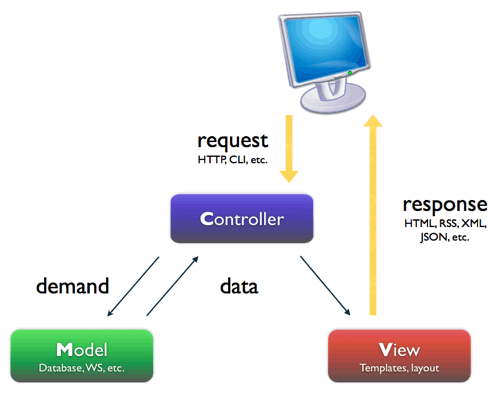
\includegraphics[width=8cm]{./images/mvc.png}
	\caption{Modelo-Vista-Controlador} \label{fig:MVC}
\end{figure}

Durante la etapa de análisis y estudio de campo se empezó diseñando en Ruby on Rails \cite{URL:Rails}, otro framework en lenguaje Ruby, sin embargo, uno de los requisitos era que la aplicación sea soportada bajo JRuby. Durante las pruebas muchas de gemas utilizadas en Rails presentaban problemas de incompatibilidad por lo que había que bajarlas de versión, y esto a su vez con otras y la aplicación. Es el caso de la \emph{gema ActiveRecord}. 

\begin{figure}[H]
	\centering
	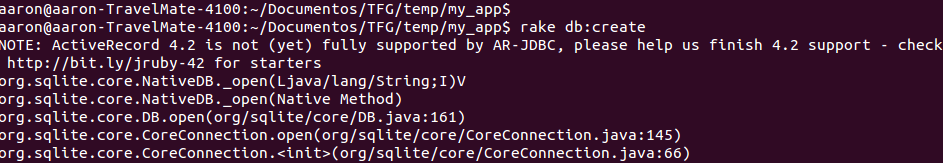
\includegraphics[width=12cm]{./images/activerecord-message.png}
	\caption{ActiveRecord 4.2 no está soportado completamente por JRuby} \label{fig:AvtiveRecord-no-supported}
\end{figure}

La idea de la compatibilidad con JRuby se considera importante para este proyecto no solo para ampliar el soporte de la aplicación, también en futuros módulos como el desarrollo en plataformas móviles o tablets con \href{http://ruboto.org/}{Ruboto}, cuyas apps pueden ser desarrolladas usando JRuby, MRI o Rubinius. \\

Por esta razón, y la libertad en diseño de la aplicación que proporciona Sinatra frente a Rails, así como su sencilla puesta en marcha, se optó finalmente por este framwork para el desarrollo de Chefmanagament. La estructura que se diseñó es la siguiente (también puede verse en \cite{URL:GitHub}):

\begin{itemize}
	\item \textbf{app}: la codificación modelo-vista-controlador se encuentra aquí. Contiene el modelo, el contolador y las vistas de la aplicación, así como funciones auxiliares (helpers) y los tests.
		\begin{itemize}
			\item config.yml: contiene los tokens e identificadores para las distintas APIs y correo usado por la aplicación.
			\item controllers: gestiona la aplicación en función de las peticiones del usuario e interactúa con el modelo y las vistas (salida al usuario).
			\item helpers: son funciones auxiliares definidas específicamente para esta aplicación. Cabe destacar el uso de la gema \href{https://github.com/mikel/mail}{Mail} para la gestión de acceso, registro y notificaciones de la aplicación.
			\item models: diseño de la base de datos. Más información en la sección~\ref{cap.2.6}
			\item tests: la definición y declaración de las pruebas. Además de comprobar las funciones y métodos creados, se ha utilizado la herramienta \href{http://www.seleniumhq.org/}{Selenium} para interactuar con la propia aplicación y pornerla a prueba. Puede ver los resultados en \href{https://travis-ci.org/alu0100207385/ChefManagement?branch=testing}{Travis}.
			\item views: su función es interactuar con el usuario, es el resultado de las acciones del usuario con la aplicación, en un formato que éste pueda entener, como páginas webs.
		\end{itemize}
	\item \textbf{public}:
		\begin{itemize}
			\item css: el estilo de las vistas.
			\item js: los archivos javascripts que controlan las entrada de datos e informan al usuario.
			\item uploads: está destinada a almacenar los archivos importados y exportados de las listas de recetas de cada usuario.
			\item resources: carpeta para almacenar recursos como imágenes, etc.
			\item otros: otras carpetas de apis usadas en la aplicación.
		\end{itemize}
	\item .travis.yml: archivo de configuración para realizar las pruebas de la aplicación en un servidor remoto. Se trata de un modelo de integración continua. Se configuró de forma que se realizaran las pruebas en distintos navegadores: Firefox (por defecto) y Chrome.
	\item Gemfile: contiene las gemas configuradas en los distintos entornos (desarrollo, producción y tests) para que la aplicación pueda funcionar.
	\item Procfile: archivo de configuración de inicio del servidor en las nubes de producción.
	\item Rakefile: contiene las distintas tareas y opciones que se pueden realizar. 
	\item config.ru: inicia la aplicación bajo \emph{rackup}.
\end{itemize}
